%mark = star, diamond, square, otimes
%\documentclass{article}
%\usepackage{pgfplots}
%\usepackage[justification=centering]{caption}
%\pgfplotsset{compat=newest}
%\begin{document}
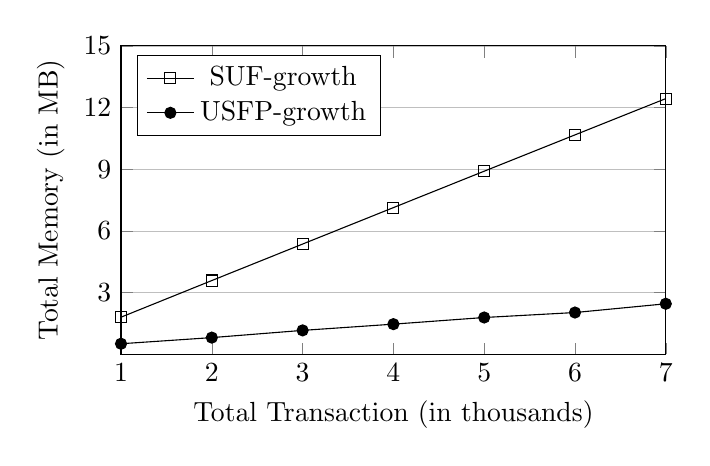
\begin{tikzpicture}
\begin{axis}[
    width=8.5cm,
    height=5.5cm,
    xlabel={Total Transaction (in thousands) },
    ylabel={Total Memory (in MB) },
    xmin=1, xmax=7,
    ymin=0, ymax=15,
    xtick={1,2,3,4,5,6,7},
    ytick={3,6,9,12,15},
    legend pos=north west,
    ymajorgrids=true,
    grid style={line width=.2pt,draw=gray!50},
]
 
\addplot[
    solid, every mark/.append style={solid, fill=gray}, mark=square
    ]
    coordinates {
			(1,1.807  )
			(2,3.588  )
			(3,5.362  )
			(4,7.134     )
			(5,8.905  )
			(6,10.670 )
			(7,12.434  )



	};
    \addlegendentry{SUF-growth}
\addplot[
    solid, every mark/.append style={solid, fill=black}, mark=*
    ]
    coordinates {
			(1,.5152  )
			(2,.814  )
			(3,1.165 )
			(4,1.468 )
			(5,1.791  )
			(6,2.033 )
			(7,2.458 )


};
    \addlegendentry{USFP-growth}
 
\end{axis}
\end{tikzpicture}
%\end{document}